\input{../preambule/preambule.tex}
\begin{center}
		{\Huge\titlefont\color{UGLiBlue} Luminosité d'une image}
\end{center}

Une image en niveaux de gris est composée de pixels et peut être représentée \textit{mathématiquement} par une matrice \og saturation\fg{} dont chaque coefficient est un entier entre 0 et 255.

Plus le coefficient est petit, plus le gris est sombre, ainsi 0 correspond à un pixel noir et 255 à un pixel blanc.

\begin{multicols}{2}
La matrice
$$\begin{pmatrix}
255&255&0&128\\
255&255&0&0\\
204&165&128&64\\
\end{pmatrix}$$

correspond à l'image ci-contre.
\columnbreak
\begin{center}
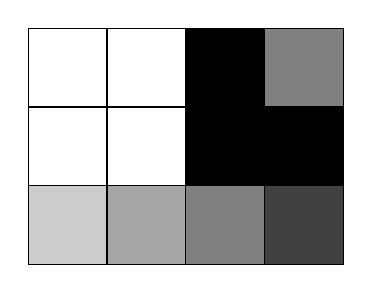
\begin{tikzpicture}
\draw[fill=black!0] (0,2) rectangle (1,3);
\draw[fill=black!0] (1,2) rectangle (2,3);
\draw[fill=black!100] (2,2) rectangle (3,3);
\draw[fill=black!50] (3,2) rectangle (4,3);
\draw[fill=black!0] (0,1) rectangle (1,2);
\draw[fill=black!0] (1,1) rectangle (2,2);
\draw[fill=black!100] (2,1) rectangle (3,2);
\draw[fill=black!100] (3,1) rectangle (4,2);
\draw[fill=black!20] (0,0) rectangle (1,1);
\draw[fill=black!35] (1,0) rectangle (2,1);
\draw[fill=black!50] (2,0) rectangle (3,1);
\draw[fill=black!75] (3,0) rectangle (4,1);
\end{tikzpicture}
\end{center}
\end{multicols}
\section*{\'Etape 1}

Voici l'algorithme d'une fonction qui crée une matrice $3\times 4$ (3 lignes de 4 colonnes).\\
La matrice est représentée par une liste de listes, chacun de ses coefficients est saisi par l'utilisateur. La fonction
\begin{enumerate}[--]
	\item ne prend rien en entrée;
    \item renvoie une liste de listes d'entiers.
\end{enumerate}
\begin{algo}    
fonction saturation_matrice()
    
    variables
        i,j, nombre : entiers # i compte les lignes, j les colonnes
        saturation  : liste  # en fait liste de listes d'entiers

    saturation ← [[0, 0, 0, 0], [0, 0, 0, 0], [0, 0, 0, 0]]
    pour i allant de 0 à ...... faire
        ......
            tant que nombre > 255 ou nombre < 0 faire
                lire nombre
            fin tant que
            saturation[i][j] ← nombre
        fin pour
    fin pour
    renvoyer saturation
\end{algo}

\begin{encadrecolore}{Question 1}{UGLiOrange}
Compléter les pointillés pour que la fonction remplisse son rôle.
\end{encadrecolore} 


La fonction suivante, nommée \mintinline{pseudocode}{luminosite} :
\begin{enumerate}[--]
	\item prend en entrée une liste de listes d'entiers \texttt{matrice}, qui représente une matrice $3\times 4$;
    \item renvoie un entier \texttt{lumi}.
\end{enumerate}

\begin{algo}    
fonction luminosite(matrice)
    
    variables
        i,j, somme, luminosite : entiers 

    somme ← 0
    pour i allant de 0 à 2 faire
        pour j allant de 0 à 3 faire
            somme ← somme + matrice[i][j]
        fin pour
    fin pour
    lumi ← partie_entiere(somme/12) # exemple : partie_entiere(3.4)=3
    renvoyer lumi
\end{algo}

\begin{encadrecolore}{Question 2}{UGLiOrange}
Lorsque \mintinline{pseudocode}{M=[[0, 0, 100, 50], [0, 70, 100, 100], [20, 35, 50, 75]]}, quelle est la valeur de \mintinline{pseudocode}{luminosite(M)} ?
\end{encadrecolore} 


Pour accentuer le contraste de l'image représentée par une matrice M, on modifie chacune des valeurs de cette matrice comme ceci :
\begin{enumerate}[--]
	\item d'abord on utilise la valeur \mintinline{pseudocode}{luminosite(M)} calculée précédemment que l'on note \mintinline{pseudocode}{lumi}.
    \item Pour chacune des 12 valeurs de la matrice M
    \begin{enumerate}[--]
    	\item si elle est inférieure ou égale à \mintinline{pseudocode}{lumi} on la divise par 2 et on garde la partie entière du résultat;
        \item sinon on la multiplie par 2 sans dépasser 255 (si la nouvelle valeur dépasse 255, on la ramène à 255).   
    \end{enumerate}    
\end{enumerate}

\begin{encadrecolore}{Question 3}{UGLiOrange}
\'Ecrire l'algorithme (ou le code \textsc{Python}) de la fonction \tw{contraste} qui 
\begin{enumerate}[--]
	\item prend en entrée une liste de listes d'entiers \texttt{matrice}, qui représente une matrice $3\times 4$;
    \item renvoie une \textit{autre} matrice : la matrice d'entrée avec un contraste accentué.
\end{enumerate}

\end{encadrecolore} 

\section*{\'Etape 2}

Le fichier \texttt{luminosite.py} contient une variable \texttt{M} représentant la matrice de la question 2 de l'étape 1.


\begin{encadrecolore}{Question 4}{UGLiOrange}
Implémenter la fonction \texttt{luminosite}.\\
Pour prendre la partie entière d'une valeur \pythoninline{v}, on pourra utiliser \pythoninline{int(v)}.
\end{encadrecolore} 

\begin{encadrecolore}{Question 5}{UGLiOrange}
Implémenter la fonction \texttt{contraste}.
\end{encadrecolore} 

\begin{encadrecolore}{Question \textsc{bonus}}{UGLiOrange}
Implémenter la fonction \pythoninline{matrice_aleatoire} qui
\begin{enumerate}[--]
	\item en entrée prend 2 entiers \pythoninline{n} et \pythoninline{p};
    \item renvoie une matrice $n\times p$ dont tous les coefficients sont des nombres aléatoires entre 0 et 255.
\end{enumerate}
On utilisera \pythoninline{from random import randint}.\\
\pythoninline{randint(a,b)} renvoie un nombre entier au hasard, compris entre \pythoninline{a} et \pythoninline{b}.
\end{encadrecolore} 
\end{document}
